\documentclass{beamer}
\usetheme{Copenhagen}

\title{The Euler Spiral}
\author{Max Mussavian}
\date[2022]{16th May 2022}
\begin{document}
\begin{frame}[plain]
    \maketitle
\end{frame}
\begin{frame}{Outline}
	\begin{itemize}
		\item Definitions and Derivations: parametric curves, lengths and curvature
		\item Relating curvature to the curve length
		\item Calculating arc length integrals
		\item Plotting the Euler spiral and other fun curves
		\item Application: designing railways and roads
	\end{itemize}
\end{frame}


\begin{frame}{Parametric curves}
	
		All curves in this talk are in $\mathbb{R}^2$.
		\begin{definition}[Parametric curve]
			A parametric curve is a smooth function that is defined on an open interval $(a, b)$ and takes values in $\mathbb{R}^2$ of the form $(x(t), y(t))$.
			\newline
			The set of points traced out by the curve is called the \textbf{trace}.
		\end{definition}
\end{frame}

\begin{frame}{Length of a curve segment}
	\begin{figure}
		\centering
		\includegraphics[width=70mm, scale=0.2]{curve_length_2.png}
	\end{figure}
	\begin{itemize}
		\item When $\Delta t = t_2 - t_1$ is small
		\item $\Delta s \approx	\sqrt{\left(\Delta x\right)^2 + \left(\Delta y\right)^2} $
		\item $\frac{\Delta s}{\Delta t} \approx	\sqrt{\left(\frac{\Delta x}{\Delta t}\right)^2 + \left(\frac{\Delta y}{\Delta t}\right)^2 } $
	\end{itemize}
\end{frame}

\begin{frame}{Length of a curve}
		\begin{itemize}
		\item As $\Delta t \to 0$
		\[
			\frac{ds}{dt} = \sqrt{\left( \frac{dx}{dt} \right)^2 + \left( \frac{dy}{dt}\right)^2}
		\]
		\item Integrate with respect to $t$ 
		\[
		s =\int_{a}^{b} \sqrt{x'(t)^2 + y'(t)^2}dt
		\]
		where $x'(t) = \frac{dx}{dt}$ and $y'(t) = \frac{dy}{dt}$
		\end{itemize}
	\begin{theorem}[Arc Length]
		The arc length between two points, $t = a$ and $t = b$, on the curve is given by
		$s =\int_{a}^{b} \sqrt{x'(t)^2 + y'(t)^2}dt$
	\end{theorem}	
  
\end{frame}

\begin{frame}{Deriving formula for curvature}
	\begin{columns}
		\begin{column}{0.4\textwidth}
			\begin{figure}
				\centering
				\includegraphics[width=50mm, scale=0.4]{curvature_illustration.png}
			\end{figure}
		\end{column}
		\begin{column}{0.6\textwidth}
			\begin{itemize}
				\item Firstly curvature is 1/radius of the osculating circle.
				\item Or the rate of change of the angle the tangent makes with the x axis with respect to arc length.
				\item $ds=rd\theta$ $\implies$ $\frac{1}{r}=\frac{d\theta}{ds}$
				
				\item From arc length 
				\begin{equation} \label{eq:1}
					\frac{ds}{dt} = \sqrt{x'(t)^2+y'(t)^2} 
				\end{equation}
				
				
			
			\end{itemize}
			
			
			
		\end{column}
	\end{columns}

	
\end{frame}

\begin{frame}{Deriving formula for curvature}
	\begin{columns}
		\begin{column}{0.35\textwidth}			
			\begin{figure}
				\centering
				\includegraphics[width=60mm, scale=0.65]{curvature_illustration_2.png}
			\end{figure}
		\end{column}
		\begin{column}{0.75\textwidth}			

			\begin{itemize}
				\item $\tan \theta = \frac{y'(t)}{x'(t)}$ 
				\item Differentiate w.r.t. $t$ gives $\sec ^2 \theta \frac{d\theta}{dt} = \frac{x'(t) y''(t) - y'(t) x''(t)}{x'(t)^2}$
				where $x''(t)=\frac{d^2 x}{dt^2}$ and $y''(t)=\frac{d^2 y}{dt^2}$
				\item $sec^2\theta = tan^2\theta +1 = \frac{{x'(t)^2+y'(t)^2}}{x'(t)^2}$ 
				\item Therefore
				\begin{equation} \label{eq:2}
				\frac{d\theta}{dt}=\frac{x'(t) y''(t) - y'(t) x''(t)}{x'(t)^2+y'(t)^2}
				\end{equation}

			\end{itemize}
	\end{column}
\end{columns}
\end{frame}

\begin{frame}{Deriving formula for curvature}
	\begin{itemize}
		\item Combining equations \ref{eq:1} and \ref{eq:2} gives us
		\begin{eqnarray*}
			\frac1r &=& \frac{d\theta}{ds} \\
					&=& \frac{d\theta/dt}{ds/dt}  \\
			        &=& \frac{x'(t) y''(t) - y'(t) x''(t)}{\left(x'(t)^2 + y'(t)^2 \right)^{3/2}}
		\end{eqnarray*}
		
		\item Curvature, $\kappa = \frac1r$
	\end{itemize}
	
\end{frame}

\begin{frame}{How curved is a curve?}
	\begin{Theorem}[Curvature]
		The curvature of curve is $\kappa$ which is the reciprocal of the radius of the osculating circle given by
		\[
		\kappa=\frac{x'(t) y''(t) - y'(t) x''(t)}{\left( x'(t)^2 + y'(t)^2 \right)^{3/2}}
		\]
	\end{Theorem}
	\begin{figure}
	\centering
	\includegraphics[width=50mm, scale=0.4]{Curvature_circle.png}
\end{figure}
\end{frame}

\begin{frame}{Curvature of a circle}
	\begin{itemize}	
		
		\item Circle: The parametric equations for a circle with radius $r$ are $x(t)=r \cos(t)$ and $y(t)= r \sin(t)$. 
		\item The arc length is 
		
		\[	
		s = \int_{0}^{2 \pi} \sqrt{r^2 \sin^2 t + r^2 \cos^2 t}dt = \left[r \right]_{0}^{2 \pi} = 2 \pi r
		\]
	
		\item Using the same parametrisations we can work out the curvature
		
		\[
		\kappa = \frac{r^2 \sin^2 t + r^2 \cos^2 t}{\left(r^2 \sin^2 t + r^2 \cos^2 t \right) ^ \frac{3}{2}} = \frac{1}{r}
		\]
		
	\end{itemize}
\end{frame}

\begin{frame}{Parabola curve length}
	\begin{itemize}	
			
			\item Parabola: For parabola $y=x^2$ the parametric equations are $x(t)=t$ and $y(t)=t^2$. The arc length between 0 and 1 is 
			\begin{eqnarray*}
				s &=& \int_{0}^{1} \sqrt{1+4t^2}dt \\ &=& \left[\frac{1}{2} t\sqrt{1+ 4 t^2} +\frac{1}{4} \ln \left(2 t+\sqrt{1+ 4 t^2} \right) \right]_{0}^1 \\
				&\approx&	 1.48
			\end{eqnarray*}
		
	\begin{figure}
		\centering
		\includegraphics[width=50mm, scale=0.4]{Parabola_Arc_Length.png}
	\end{figure}
	\end{itemize}
\end{frame}

\begin{frame}{Parabola curvature}
	\begin{itemize}	
		
		\item Parabola: Recall $x(t)=t$ and $y(t)=t^2$. 
		
		\[
		\kappa = \frac{2}{\left(1 + 4t^2 \right) ^ \frac{3}{2}}
		\]
		
	\begin{figure}
	\centering
	\includegraphics[width=50mm, scale=0.4]{Parabola.png}
\end{figure}

	\end{itemize}
\end{frame}

\begin{frame}{Relating curve length to curvature}
	Let's try the following parametrisation for $x$ and $y$
	\begin{eqnarray*}
		x(t) &=& \int_{0}^{t} \cos f(u) du \\
		y(t) &=& \int_{0}^{t} \sin f(u) du
	\end{eqnarray*}
	This gives us
	\begin{eqnarray*}
		x' = x'(t) = \cos f(t) &\mbox{ and }& x''=-f'(t) \sin f(t) \\
		y' = y'(t) = \sin f(t) &\mbox{ and }& y''=f'(t) \cos f(t)
	\end{eqnarray*}
\end{frame}

\begin{frame}{Relating curve length to curvature}
	The slope, arc length and curvature now are:
	\begin{eqnarray*}
	\frac{dy}{dx} &=& \frac{\sin f(t)}{\cos f(t)} = \tan f(t) \\
 	s &=& \int_0^t \sqrt{\cos^2 f(u) + \sin^2 f(u)} du = t \\
 	\kappa &=& \frac{f'(t) \cos^2 f(t) + f'(t) \sin^2 f(t)}{\cos^2 f(t) + \sin^2 f(t)} = f'(t)
 \end{eqnarray*}
	\begin{enumerate}
		\item We can replace the variable $t$ by arc length $s$.
		\item And curvature at point $t$ is $f'(t)$. 
	\end{enumerate}
\end{frame}

\begin{frame}{Define the curve by curve length and curvature}
	 This all implies
	 \[
	 f(u) = \int_{0}^{u} \kappa(t) dt
	 \]
	Thus the equations for the curve become
	\begin{eqnarray*}
	x = x(s) &=& \int_{0}^{s} \cos \left( \int_0^u \kappa(t) dt \right) du \\
	y = y(s) &=& \int_{0}^{s} \sin \left( \int_0^u \kappa(t) dt \right) du
	\end{eqnarray*}
	Hence the curve is defined by arc length and curvature alone!
\end{frame}

\begin{frame}{A very simple example}
	Suppose the curvature $\kappa$ constant and equal to 1. 
	\linebreak
	\linebreak
	Then 
	$ \int_0^u \kappa(t) dt = u $ and
	\begin{eqnarray*}
		x = x(s) &=& \int_{0}^{s} \cos u du = \sin s\\
		y = y(s) &=& \int_{0}^{s} \sin u du = - \cos s + 1
	\end{eqnarray*}
	which is the parametric curve for a circle with centre $(0, 1)$ and radius $1$ - as expected.
	
\end{frame}


\begin{frame}{The Euler spiral}
	Euler defined his curve as one where the curvature is proportional to arc length.
	
	\begin{center}
		\boxed{\kappa(s) = s}
	\end{center}
	Then 
	$ \int_0^u \kappa(t) dt = \frac{u^2}{2} $ and
	\begin{eqnarray*}
		x = x(s) &=& \int_{0}^{s} \cos \frac{u^2}{2} du\\
		y = y(s) &=& \int_{0}^{s} \sin \frac{u^2}{2} du
	\end{eqnarray*}

	But since these integrals can't be solved analytically how were they calculated?
\end{frame}

\begin{frame}{Solving the integrals: Euler}
	\begin{itemize}
		\item In 1744 Euler derived these integrals.
		\includegraphics[width=50mm, scale=0.5]{euler_scripture_1.png}	
		\item He derived a series expansion which is still a viable method for small $s$.
		
		\includegraphics[width=100mm, scale=0.7]{euler_scripture.png}
		
		\item In 1781 he proved the integrals for limits between 0 and $\infty$ are equal to  $\frac{a \sqrt{\pi}}{2}$ where $a=1$ for the Euler spiral.
	\end{itemize}
\end{frame}

\begin{frame}{Solving the integrals: Fresnel}
	\begin{itemize}
		\item Fresnel rediscovered these integrals when investigating the diffraction of light through a slit. He showed that the light intensity (under some assumptions) was 
		\[
		\left( \int_{0}^{s}\cos \left( \pi t^2 / 2 \right) dt \right) ^2 + 
		\left( \int_{0}^{s}\sin \left( \pi t^2 / 2 \right) dt \right) ^2
		\] 
		\item These integrals are the same as the ones Euler derived (up to a factor of $\pi$).
		\item Integrals are called the \emph{Fresnel integrals}.
		\item Fresnel calculated them for values of $s$ between 0.1 and 5.1.
	\end{itemize}
\end{frame}

\begin{frame}{Solving the integrals: using Python}
	\begin{columns}
		\begin{column}{0.5\textwidth}
			\includegraphics[width=50mm, scale=0.5]{code_1.png}
			
			\includegraphics[width=50mm, scale=0.5]{code_2.png}
		\end{column}
		\begin{column}{0.5\textwidth}
		Nowadays computers and numerical methods are used to evaluate these integrals.
		\end{column}
	\end{columns}
\end{frame}

\begin{frame}{The Euler spiral - $x$ $y$ Coordinates}
	\begin{figure}
		\caption{Fresnel integrals with arguments $\frac{u^2}{2}$}
		\centering
		\includegraphics[width=70mm, scale=0.5]{euler_x_vs_y.png}
	\end{figure}
	As expected these converge to $\pm \frac{\sqrt{\pi}}{2} \approx 0.8862$.
\end{frame}

\begin{frame}{The Euler Spiral}
	\begin{figure}
		\caption{The Euler spiral aka Cornu spiral}
		\centering
		\includegraphics[width=70mm, scale=0.5]{euler_spiral.png}
	\end{figure}
	
\end{frame}

\begin{frame}{Eulers first drawing}
\begin{figure}
	\centering
	\begin{minipage}{.5\textwidth}
		\centering
		\includegraphics[width=.8\linewidth]{Euler_first_drawing.png}
		\caption{Euler's first drawing from a 1744 publication. P refers to a weight.}
		\label{fig:test1}
	\end{minipage}%
	\begin{minipage}{.5\textwidth}
		\centering
		\includegraphics[width=0.9\linewidth]{Euler second drawing.png}
		\caption{Euler's drawing of full spiral in 1781 after solving integrals to $\infty$}
		\label{fig:test2}
	\end{minipage}
\end{figure}
\end{frame}

\begin{frame}{Other fun curves: even powers of $s$}
	\begin{figure}
		\caption{$\kappa(s) = s^2$}
		\centering
		\includegraphics[width=85mm, scale=0.5]{chaise_longue.png}
	\end{figure}
\end{frame}

\begin{frame}{More fun curves: mix in a bit of a circle}
	\begin{figure}
		\caption{$\kappa(s) = s ^ 2 -2.19$}
		\centering
		\includegraphics[width=35mm, scale=0.2]{s_squared_minus_219.png}
	\end{figure}
\end{frame}

\begin{frame}{More fun curves: polynomials}
	\begin{figure}
		\caption{$\kappa(s) = 5 s ^ 4 - 18 s ^ 2 + 5$}
		\centering
		\includegraphics[width=70mm, scale=0.5]{five_s^4.png}
	\end{figure}
\end{frame}

\begin{frame}{More fun curves: trigonometric functions}
	\begin{figure}
		\caption{$\kappa(s) = \cos(s) - s \sin(s)$}
		\centering
		\includegraphics[width=50mm, scale=0.2]{elegant_madness.png}
	\end{figure}
\end{frame}
	
\begin{frame}{More fun curves: hyperbolic functions}
	\begin{figure}
		\caption{$\kappa(s) = \sinh(s) - 5.19$}
		\centering
		\includegraphics[width=100mm, scale=0.5]{sinh.png}
	\end{figure}
\end{frame}

\begin{frame}{Application: Designing roads and railways}
	\begin{itemize}
		\item Euler's spiral was rediscovered by railway designers in the 19th century.
		\item Transition curves link straight sections of roads or railways.
		\item Designed to give passengers a smooth ride with no sudden changes in acceleration.
	\end{itemize}
	\begin{figure}
		\caption{Cloverleaf motorway interchange}
		\centering
		\includegraphics[width=40mm, scale=0.5]{cloverleaf_motorway.png}
	\end{figure}

\end{frame}

\begin{frame}{Why transition curves are Euler spirals}
	\begin{itemize}
	\item Acceleration along a transition curve is
 	 \[
 	 a=s''(t) \vec{T}+\kappa s'(t)^2 \vec{N}
 	 \]
 	 where $\vec{T}$ is the unit tangent vector and $\vec{N}$ is the unit normal vector, $s(t)$ is the curve length, $s'(t) = \frac{ds}{dt}$ and $s''(t) = \frac{d^2 s}{dt^2}$.
 	 \item If the car/train is going round the curve at constant speed $s'(t)=constant$ and $s''(t)=0$.	
 	 \item The acceleration at constant speed depends on the curvature $\kappa$ and speed $s'(t)$ in the direction of the normal vector.
 	 \item For smooth ride curvature should increase with curve length.
	\end{itemize}
\end{frame}

\begin{frame}{Case 1: Semicircular transition curves}
	A closed  track is made up of four segments.
	\begin{enumerate}
		\item A straight track of length 1km
		\item A semicircular track of length 1km. This has radius $1,000 / \pi m \approx 318.31m$
		\item A straight track of length 1km
		\item A semicircular track of length 1km.
	\end{enumerate}
	Let the vehicle go around the track at a constant speed of $60 km/h = 16 \frac{2}{3} m/s$.
\end{frame}

\begin{frame}{Case 1: Position and acceleration}
	\begin{columns}
		\begin{column}{0.8\textwidth}			
			\begin{figure}
				\caption{Position and acceleration}
				\centering
				\includegraphics[width=70mm, scale=0.2]{circular_track.png}
			\end{figure}
		\end{column}
		\begin{column}{0.33\textwidth}
			Note: Acceleration is a step function. 
			
			As a passenger you feel the full centrifugal force ($F=mv^2/r$) pushing you outward the moment you entered the curve. 		
		\end{column}
	\end{columns}
\end{frame}


\begin{frame}{Case 2: Euler spiral transition curves}
	\begin{itemize}
		\item A closed track with same width and height. 
		\item Replace semicircles with two half Euler Spirals.
		\item Curvature is proportional to arc length: $\kappa(s) = \alpha s $ for some $\alpha$.
		\item Width and height of an Euler Spiral that turns through $\pi/2$ is 
		\begin{eqnarray*}
			width &=& \sqrt{\pi / \alpha} C(1) \\
			height &=& \sqrt{\pi /\alpha}S(1)
		\end{eqnarray*}
		where $S(u)$ and $C(u)$ are the standard Fresnel integrals.
	\end{itemize}
	\[
		\alpha = \frac{\pi S(1)^2}{r^2} \approx 5.95 \times 10 ^{-6}
	\]
	
\end{frame}

\begin{frame}{Case 2: Euler spiral transition curves}
	\begin{columns}
		\begin{column}{0.8\textwidth}			
			\begin{figure}
				\caption{Position and acceleration}
				\centering
				\includegraphics[width=70mm, scale=0.2]{euler_track.png}
			\end{figure}
		\end{column}
		\begin{column}{0.33\textwidth}
			Note: Acceleration increases linearly as we move through the curve.
			
			The maximum acceleration at the apex is greater than with the semicircular track but the ride is now more comfortable.
					
		\end{column}
	\end{columns}

\end{frame}



\begin{frame}
	\centering
	Thanks for listening!
	 
\end{frame}

\end{document}
